\chapter{Methods} % Main chapter title

\label{chap:methods} % For referencing the chapter elsewhere, use \ref{Chapter1} 

%----------------------------------------------------------------------------------------

To address of problem of localizing cortical areas processing semantic \similarity and / or \association, we use voxel-wise fMRI encoding to estimate local superiority of semantic representations. The human subjects' brain activity are recorded when they attentively listen to naturally spoken narrative stories from \citetitle{saint-exuperyPetitPrince1943}. We construct features (regressors) using non-semantic signals (including acoustic energy, word presence and content word presence) and semantic representation models tuned for semantic \similarity and \association. 

\section{fMRI Acquisition and Preprocessing}
\label{sec:fmriAcquAndPrepro}

The fMRI experiment is designed and carried out by \textcite{todorovicAnalysesIRMfLors2018}. 20 French native speakers (11 females, average age of 24.5 years-old, range 18-39 years-old, right handed according Edinburgh's inventory \parencite{oldfieldAssessmentAnalysisHandedness1971a} (adapted for French, averaged score 0.903, range 0.375-1), without antecedent neurological or psychiatric disorders) were recruited from Neurospin's volunteer inventory. The participants listened to the French audio book \citetitle{desaint-exuperyLittlePrinceFrench2011} \parencite{desaint-exuperyLittlePrinceFrench2011} during 9 runs. They were tested with comprehension multi-choice questions at the end of each block. During the listening period, a Siemens scanner scanned the whole brain at 3 Tesla with multi-echo EPI sequence at 2 second-per-image rate. Each scanning session (run) lasted at maximum 90 minutes. Each subject passed all the recording during the same day. 

The multi-echo procedure has a higher signal-to-noise ratio over mono-echo. Therefore, activities in traditionally unaccessible cortical areas such as the ventral temporal cortex. The voxel size, as a compromise, is fixed at a larger volume than classic modern fMRI recordings of  \(3.159 \times 3.159 \times 3.159 mm ^ 3\). The acquired MRI (anatomical and functional) data are then preprocessed with ME-ICA pipeline\footnote{Library available at \url{https://github.com/ME-ICA/me-ica}, commit \code{6ae63c7}.} \parencite{kunduDifferentiatingBOLDNonBOLD2012} to transform spatial normalization to MNI template and extract whole-brain BOLD signals. 

Please refer to appendix Section \ref{appsec:stimuliAndControl} for comprehension question designs and fMRI stimuli preprocessing, Section \ref{appsec:fmriacquisition} for more detailed participant recruitment, fMRI procedure presentations, and to the original report (in French) \parencite{todorovicAnalysesIRMfLors2018} for original materials used in the experiment.

\section{Semantic Feature Embedding Construction}

To build regressors for voxel models of different semantic processing axes, we first obtain corresponding semantic embedding of the semantic principles in question. We then validate the embedding performances in \similarity and \association semantic proximity ranking evaluations before being used to build fMRI regressors.

Since we do not have widely-used French evaluation task benchmarks in disposition, our implementation of semantic embedding algorithms are tuned and validated firstly on English data, then transferred on French data. 


\subsection{Semantic Similarity Embedding}
\label{subsec:semanticsimilaritymethod}
To build semantic similarity representation, English \code{WordNet}\footnote{Version 3.1, available at \url{https://wordnet.princeton.edu/download/current-version}} \parencite{millerWordNetLexicalDatabase1995, millerWordNetElectronicLexical1998}, French \code{WOLF} \parencite{sagotBuildingFreeFrench2008} serve as our data source. For semantic entities encoded in an ontological graph with internal semantic relations, \textcite{saediWordNetEmbeddings2018} proposed an evaluation of semantic affinity by counting all the paths connecting two nodes representing entities. The paths are indexed by semantic relationships, and are weighted by their length: shorter is the path, stronger is the semantic affinity. Equation \ref{eqn:randomwalk} illustrates the exact numerical calculation by taking \(M\) as the weighted adjacency matrix representation of the initial graph. 
\begin{equation}
    M_G^{(n)} = I + \alpha M + \alpha^2 M^2 + \dots + \alpha^n M^n \\
    M_G = \sum_{e=0}^{\infty}{(\alpha M)}^e = (I - \alpha M)^{-1}
\label{eqn:randomwalk}
    \end{equation}

After computing the graph distance of between all word-pairs, a normalized Positive Point-wise Mutual Information transformation is applied to the matrix to reduce noises introduced by unbalanced word occurrence frequency. Finally a PCA is performed to reduce the dimensionality of the large matrix. 

We replicated \citeauthor{saediWordNetEmbeddings2018}'s experiment using the reported optimal parameters\footnote{including graph random-walk decay factor, semantic relation weight attribution}. Our tests differed from the original work's configuration on semantic relation selection, vocabulary size and dimensionality choice of the resulting embedding space. 

As mentioned in the Section \ref{subsection:hypsemantichub}, typical similarity-related relationships include synonymy, hypernymy, hyponymy. In \code{WordNet} implementation, we extend these relationships to include also the relation where an adjective is a participle of verbs (e.g. \emph{exhausting} is a participle of \emph{exhaust}), is similar to another adjective (\emph{exhausting} and \emph{tiring} are similar to \emph{effortful}) and where an adverb is derived from an adjective (\emph{essentially}, \emph{basically} and \emph{fundamentally} are derived from \emph{essential}). We test different set of combinations of relations to further confirm our choice for \similarity and \association classification (see Section \ref{appsubsec:wnembeddingtests}).

As large matrix calculation is very memory-consumptive, given the available memory on the laboratory server\footnote{The computer is equipped with an quad-core Intel Xeon processors @ \code{3.70 GHz}, \code{32 GB} RAM, running Ubuntu \code{18.10}, Python \code{3.6.7} Anaconda.}, we selected the 15 000 most frequent words in \code{WordNet} and 20 000 in \code{WOLF} for fast in-memory computing, and then took 60 000 in \code{WordNet} and all words in \code{WOLF} (56665) for optimal embedding performances. 

A balance between model complexity and precision is required. To determine the number of principle components (PC) of the graph encoding word-wise proximity, we initially keep first 8 000 PCs as potential candidate (see Figure \ref{fig:SimDimensionSeletionVarRatio}). Thresholding directly the singular values or the explained variance ratios (EVR)\footnote{EVR is the eigenvalue of the PC divided by the sum of all eigenvalues} resulted to either too few or too much retained PCs. We use the discrete derivative of the EVR to obtain second-degree information. Since the derivative is extremely noisy but a general decreasing trend could be seen, we apply a Savitzky-Golay filter\footnote{Low-degree polynomials are fitted on a subset of data points with least-square error minimization, so that data points can be smoothed without distorting the global trends} of window size 100 and of first order on the discrete derivative of EVR. The cutting position is visually selected around the first local minima with a following sufficiently wide valley of the smoothed signal (Figure \ref{fig:SimDimensionSelectionVarRatioDiff}). The derivative as the cutting basis is more sensible to information conservation in embedding spaces.

\begin{figure}
    \centering
    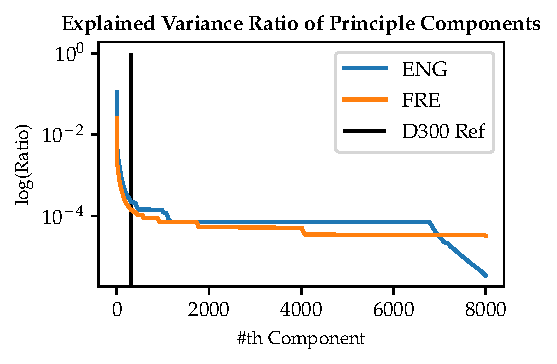
\includegraphics[scale=1]{Figures/SimDimensionSelectionVarRatio.pdf}
    \caption[Explained Variance Ratio of \code{WordNet} Embedding Principle Components]{The \code{log} of EVR of each PC in \code{WordNet} embedding space (\code{ENG}) and in WOLF embedding space (\code{FRE}). The PCs are ordered by their corresponding eigenvalues. The black vertical line is placed at the classic choice dimensionality of 300 as a reference.}
    \label{fig:SimDimensionSeletionVarRatio}
\end{figure}

\begin{figure}
    \centering
    \makebox[\linewidth]{
    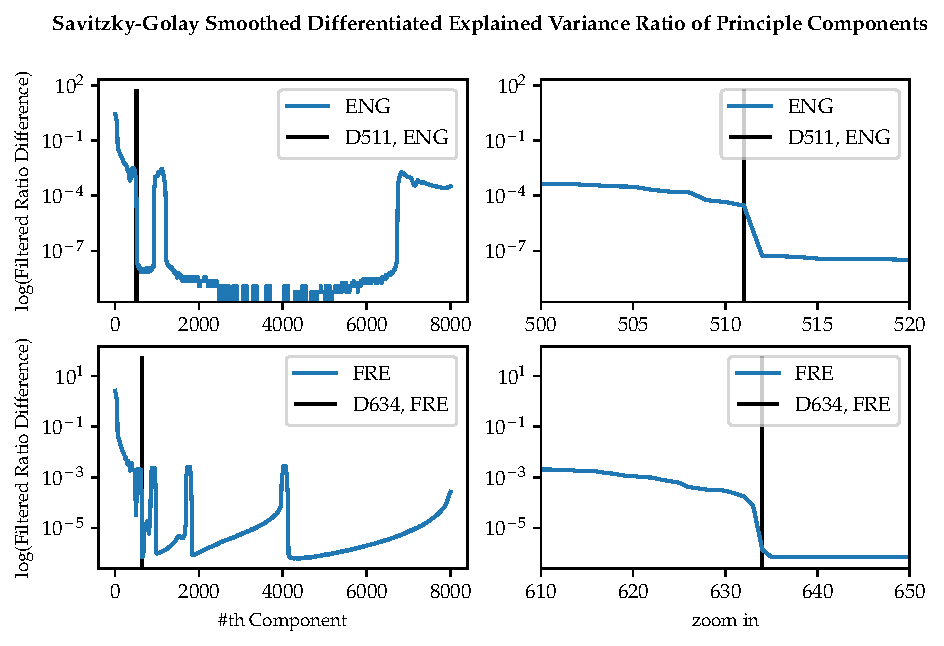
\includegraphics[width=\textwidth]{Figures/SimDimensionSelectionVarRatioDiff.pdf}
    }
    \caption[Smoothed Differentiated EVR of \code{WordNet} Embedding PCs]{\textbf{Left panels}: Savitzky-Golay filter smoothed the discrete derivative of the PC EVR signal. \code{D511} in \code{ENG} and \code{D634} in \code{FRE} are visually selected on the left border of a sufficiently wide signal valley. }
    \label{fig:SimDimensionSelectionVarRatioDiff}
\end{figure}

% code Decorrelation_French.ipynb

\subsection{Semantic Association Embedding}


\begin{equation}
    M = S.P + A 
    \label{eqn:linearmixture}
    \end{equation}

Using the linear approximation of \similarity and \association information mixture in classical SDRs (refer to Section \ref{subsection:hyplinearsemantics}), we extract \association representations from classic statistical embeddings with equation \ref{eqn:linearmixture}, where \(M\) is the mixed semantic representation space, \(S\) being the \similarity based space, \(P\) a learned projection matrix projecting the similarity space onto the mixed space, and the residual \(A\) being the \association space. The embedding spaces of interest are \(S\) and \(A\), henceforth respectively noted as \code{SIM}(short for \textbf{sim}ilarity) and \code{ASN} (\textbf{as}sociatio\textbf{n}). The two auxiliary spaces are \(P\) and \(M\), noted as \code{SIG} (\textbf{si}milarity projected on (Dep)\textbf{G}love) and \code{MIX} (\textbf{mix}ed). The projection weight \(P\) is learned via a general linear model (GLM)\footnote{\url{https://scikit-learn.org/stable/modules/linear_model.html}}, with the computational objective to minimize the L-2 norm of \(A\).

For \code{MIX} spaces, for English we use GloVe \parencite{penningtonGloveGlobalVectors2014} trained on Common Crawl with 840B tokens, 2.2M cased vocabulary and 300-dimension vectors\footnote{Pretrained data available at \url{https://nlp.stanford.edu/projects/glove/}}. For French we use DepGloVe\footnote{Pretrained data available at \url{http://alpage.inria.fr/depglove/process.pl}} \parencite{delaclergerieDepGloveSmallServer}. 

English GloVe embeddings provide word-level vectorial representations. However, since French verbs and adjectives have various inflective forms, this inflection can thin out captured semantic information if each specific form does not have sufficient frequency in a given corpus. DepGloVe aggregates semantic information by lemmatizing the tokens and attribute them with a part-of-speech (POS) tag. The main POS tags include \code{nc} (common nouns), \code{np} (proper nouns), \code{v} (verb), \code{adj} (adjectives), \code{adv} (adverbs) along with auxiliary tags.

To formulate the GLM dataset, modifications on heterogeneous embedding data are made to align the embedding spaces. Each row of the an embedding space matrix represents a lexicon unit. Since different semantic spaces have different lexicon settings, only the intersection of two vocabularies of one same language is kept in later stages. The lexicon alignment between the English embeddings is based on orthography, which is computed by string comparison. For French data, multiple text sources are converted to the same format: lemma tagged with \code{WOLF} POS tags (nouns, verbs, adjectives and adverbs). We hand coded rules to tidy up \code{WOLF} vocabulary and transformed DepGloVe's complex POS tagging entries into \code{WOLF}'s relatively simple set. Our textual data including validation task benchmarks and fMRI stimuli are also transformed to align with this strategy. Finally we manually check the vocabulary coverage against validation dataset and fMRI stimuli words, we also performed manual correction in the newly aligned space to purge algorithm erroneous results.  % code Decorrelaation_French.ipynb & Text Preprocessing.ipynb

\subsection{Embedding Validation}

Since many assumptions and approximations are made on the structure and content of semantic representation spaces, the interpretation of further results depends on the validity of the embedding construction.

The semantic ranking task depends on databases of word-pairs, each attributed with a score (usually annotated by human) which measures the proximity in terms of the semantic property defined by the task. Each semantic embedding is provided with a proximity metric, which could be derived from graph distances or vectorial distances. The score of the task is computed by calculating Pearson's and Spearman's correlation coefficient \code{r} between the embedding based word-pair proximity and the baseline. 

Conformably with other works on semantic model evaluation methods [TODO Refs, other works using the same benchmarks] \parencite{saediWordNetEmbeddings2018}, we use benchmark data provided by \textcite{rubensteinContextualCorrelatesSynonymy1965} (\textbf{RG1965}), \textcite{agirreStudySimilarityRelatedness2009} (\textbf{WS353-Similarity}) and \textcite{hillSimLex999EvaluatingSemantic2015} (\textbf{SimLex-999}) to evaluate English semantic similarity models. The only available benchmark conceived for evaluating association relations is \textbf{WS353-Association}.

\label{subsection:frenchbenchmarkdataconstruction}
\textcite{freitasSemanticRelatednessAll2016} provides translation for some of those benchmarks in French, however the provided proximity scores are heterogeneous with the original rankings. Scores for French \textbf{SimLex-99} are given by a computer semantic model, while \textbf{WS353} scores are identical with English data. The latter configuration is problematic since in different languages the translation are not exact mappings between words, and the proximities are subject to the nuanced translation choice. We manually corrected the erroneous translation of word pairs, eliminated and replaced distinct original word-pairs that are translated to the same target word-pairs, or word-pairs to the same words. Scores for the replaced word-pairs are retrieved from the English dataset. The built French benchmark data suffer from the lack of real human judgement data, thus they serve merely as indicators of semantic model performance. The modified benchmarks are made available on GitHub\footnote{commit \code{c97583f}, \url{https://github.com/nicolasying/Similarity-Association-Benchmarks}}.

\section{fMRI Voxel-Wise Encoding}


In this project and many other similar works [TODO, refs], we consider the BOLD signal of a given voxel \code{j} as a temporal signal, which is linearly composed by various independent functional sub-signals, which themselves are convolutions of separate neuron activations with a hemodynamic function: 

\begin{equation}
    \text{BOLD}_{\text{theory}, j}(t) = \sum_i {\beta_{i,j} \times f_{i}(t) * \text{hrf}(t),}
\label{eqn:boldlinear}
\end{equation}

where \(\beta_{i,j}\) is the linear coefficient of the \code{i}-th component, \(f_{i}\) is a function modeling the \code{i}-th independent functional activation, and \(\textnormal{hrf}\) is the hemodynamic function\footnote{We used packaged functions from \code{nistats, nilearn} to implement regressor construction~\parencite{abrahamMachineLearningNeuroimaging2014}.} (we use the model used in SPM at oversampling rate of 10, the hemodynamic function is illustrated in Figure \ref{fig:hrf}).

\begin{figure}
    \centering
    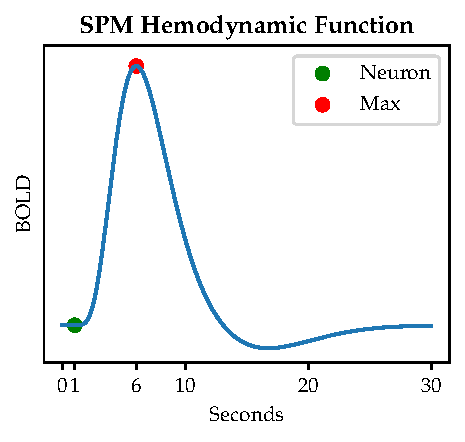
\includegraphics[scale=.8]{Figures/SPMHDF.pdf}
    \caption[SPM Hemodynamic Function]{The shape of the hemodynamic function used in the project. The modeled neural activity instantaneously fires at 1s. The maximum of the hemodynamic function is attained at 6s.}
    \label{fig:hrf}
\end{figure}


Since different voxels contain neurons of distinct (yet possibly similar) activation profiles towards stimuli, the coefficient associated with each functional component are also different for each voxel. For example, in an auditive comprehension task, the statistical distribution of GLM trained coefficients (\(\beta_{i}\) in equation \ref{eqn:boldlinear})associated to a voxel which is not implicated in audition to be near 0. Voxels containing neurons primarily associated with low-level auditive functions having non-zero \(\beta\)s for low-level auditive features.

\subsection{fMRI Textual Stimuli Preparation} 

% notebook, Text Preprocessing.ipynb
For the generation of regression features for fMRI encoding, we perform a lemmatization of the Little Prince story. First the text is parsed with syntactic dependency analysis with \code{spaCy}\footnote{version \code{2.0.16}} library and each token is attributed with a POS tag. We then used \code{FrenchLefffLemmatizer}\footnote{commit \code{ba1ef2b}. The library is publicly available on GitHub, \url{https://github.com/ClaudeCoulombe/FrenchLefffLemmatizer.}}\parencite{sagotLefffFreelyAvailable2010} library to return verbs to the infinitive form and other words to masculine singular form. POS info from \code{spaCy} helps to resolve lemmatisation ambiguity. The pipeline-generated lemma and POS tags are then manually verified and corrected\footnote{The pipeline and hand-made modifications are available at \url{https://github.com/nicolasying/Micipsa-Text-Preprocessing/blob/master/Text\%20PreProcessing.ipynb}.}.

\subsection{Regression Feature Generation}
\label{subsec:regressionfeaturegeneration}
The exact transcription of the audiobook is performed by \textcite{todorovicAnalysesIRMfLors2018}. With \code{jtrans} and \code{Praat}, the authors aligned the audio with the text by marking the onset and offset of each pronounced word in the story. To pin down the BOLD signal at a given time, we reconstruct temporal regressor functions by firstly build \(f_{i}\) in equation \ref{eqn:boldlinear}, which is essentially a sequence of bumps each occurs at the onset of a word (or content word), then we concatenate the sequence of convoluted \(D\) regressors into a design matrix of \(D\) columns.

% code TextFineTuning\LPP Onset\Lemmatisation Feature Gen.ipynb, generate_regressors.py, events2reg.py
We used four groups of features to reconstruct human listening comprehension processing cerebral activities:
\begin{enumerate}
	\item \code{RMS} (Acoustic Energy), which is the root means square of audio wave amplitude calculated on a sliding window of 10 msec, with Octave\footnote{\url{https://www.gnu.org/software/octave}}.
	\item \code{WRATE} (Word Presence), a binary temporal sequence indicating if a word is being pronounced at a given time.
	\item \code{CWRATE} (Content Word Presence), a similar binary feature to \code{WRATE}, which indicates the presence of a content word, determined by the POS tag (including nouns, verbs, adjectives and adverbs) of the lemmatised text. 
	\item \code{SIM/ASN/SIG/MIX} (Semantic Embedding-Based Features), a multi-dimensional feature set. The feature value is taken from a certain embedding defined in \(\mathbb{R}^{\vert vocabulary \vert \times n}\) space, where a particular matrix row corresponds to the content word in question. 
\end{enumerate}

\code{RMS} and \code{WRATE} are reported by post-hoc analysis of \textcite{todorovicAnalysesIRMfLors2018} as informative features. Henceforth, we define a \emph{regressor group} the regressors built from a group of features, \emph{regressor class} as the combination of regressors from the regressor group with the same name and the groups of lower feature levels. For example, the \emph{regressor class} \code{SIM} contains regressors from \emph{regressor groups} of \code{RMS}, \code{WRATE}, together with \code{SIM}.

For the ease of later design-matrix feature selection, we systematically performed orthonormalization of the convoluted feature sequences to cancel the co-linearity of the regressors. This is implemented with Gram-Schmidt process\footnote{Gram-Schmidt process is an iterative procedure applied over a set of linearly independent functions. It construct an orthogonal basis by subtracting the projection of a posteriorly positioned column over existing partial orthogonal basis (initially this basis is the first column), so that the residual of the subtracted column is linearly independent. The column residual is added to the orthogonal basis and the procedure continues until the last column is added to the basis.}~\parencite{GramSchmidtProcess2019} , where the orthogonal sequence is defined by the order of regressor classes above, and the semantic embedding based regressors inner-class order is either given by the original semantic model (\code{ASN/SIG/MIX}) or by PCA (\code{SIM}). 

\subsection{Feature Selection for Specific Corpus}
% notebook, Embedding Dimension Selection for LPP.ipynb

\code{SIM} space is constructed by taking the first PCs of a transformed ontological graph adjacency matrix, the explained variance associated to each PC is informative. As \citetitle{saint-exuperyPetitPrince1943} uses limited vocabulary, the semantic space might not be fully exploited as it was factorized with a much larger lexicon. We suspect that there might be some semantic dimensions in the semantic spaces that are not fully exhibited. It is in our interest to simplify the design matrix, leave out uninformative feature columns (those with extremely low variances) to avoid overfitting and accelerate model fitting computation. Therefore we take an investigation of the 9 design matrices (one per fMRI block) by averaging each design matrix's variance of individual regressors. After orthonormalization, the variance of regressors in higher dimension positions are of a much smaller order than the first regressors especially for PCA-factored semantic spaces. The value of threshold for column selection is determined visually to limit the number of informative regressors under 200.

\subsection{Ridge Regression with Step-wise Forward Feature Selection, Grid Search and Cross Validation}
% Ridge regression with stepwise feature selection, GridSearch Alpha 
% Github code
\label{sec:ridgemethod}
The fMRI encoding protocol is to find a function projecting our theoretical feature regressors onto BOLD amplitudes. We assume that the target BOLD value is linearly composited by individual regressors, similar in equation \ref{eqn:boldlinear}. The coefficients in the equation above is determined by the minimization of the squared difference between the predicted value given by the voxel-model and the recorded BOLD value, on a set of discrete timestamps. This is a typical regression problem tackled in Machine Learning. The computation of the coefficients is named \emph{training} or \emph{fitting} of the model. The performance of a fitted model trained on a dataset is evaluated on the accuracy of its predictions on unseen data, which indicates its \emph{generalized predictive power}.

In each fMRI recording block we have around 300 whole-brain images (refer to Section \ref{appsubsec:fmridata} for more details), totaling 2937 observations. Researchers \parencite{huaOptimalNumberFeatures2005} found that in GLM the optimal number of uncorrelated informative features is \(N - 1\) where \(N\) is the number of observation, and \(\sqrt{N}\) if features are correlated. Although we have numerically de-correlated the regressors, we nevertheless cannot assume the conceptual independency. Thus 200 regressors might outnumber the recommended feature size. To avoid potential overfitting of regression models, we use Ridge regression to penalize the attribution of large coefficients. Equation \ref{eqn:ridge} is the minimization problem posed by Ridge regression, with \code{j} fixed for voxel \code{j} and \(N_j\) the number of features used by voxel \code{j}. Strong penalization reduces potential noises by limiting the chance of particular feature columns weighing too much on final prediction, therefore promotes the robustness and generalizability of a fitted model.

\begin{equation}
    \min_{\beta_{i,j}}{\sum_{t}{\vert\sum_{i}^{N_j}{\beta_{i,j} \times f_{i}(t) * \text{hrf}(t)} - \text{BOLD}_{\text{real}, j}(t)\vert ^2} + \alpha_j \sum_{i}^{N_j}{\beta_{i,j}^2}}
\label{eqn:ridge}
    \end{equation}

Ridge regression fitting algorithm requires a hyper-parameter (\(\alpha\)) to adjust the severity of large-coefficient penalty. There's no empirically predetermined optimal choice of the value for similar project settings, thus we test a range of candidates by fitting different models and evaluate their performance. 

We also assumed the heterogeneity of voxel activation profile towards different functional features. In order to maximize the predictive power of models, we trial multiple combinations of feature columns on each voxel-model. Limited by the computation time, we do not test all the combinations of individual features which could results in an exponential complexity, but use \emph{step-wise forward} feature selection by the order of feature classes (Section \ref{subsec:regressionfeaturegeneration}). 

A major difference of this project from \textcite{todorovicAnalysesIRMfLors2018, verdierEncodageActiviteNeuronale2018} is the voxel-specific configuration. Our pilot regression experiments partially replicated the original experience \parencite{todorovicAnalysesIRMfLors2018} on French data. The results showed that fixing one regularization parameter for all models (including non-semantic models and \code{MIX} models) cannot fully exploit the power of the supplied regressors. The fixed \(\alpha\) preferentially improves the regression performance for certain models. 

By prior experiences, a search range for \(\alpha\) is fixed beforehand. We sampled 34 \(\alpha\)s from the defined range and up to 32 feature dimension candidates, in hope of including the near-optimal hyper-parameter combination for the regression of each voxel-level model. The list of tested parameters are fixed in each model's config file\footnote{For example, \code{ASN} is configured as \url{https://github.com/nicolasying/Micipsa/blob/master/models/fr/rms-wrate-cwrate-asn200/config.json}. Please refer to Section \ref{appsubsec:regressionparameters} for tested \(\alpha\) value, feature selections.}.

In our project, for each voxel of a subject and each combination of \(\alpha\) value candidate and feature selection, we adopt the common practice of Cross Validation (CV), where we generate 9 different regression models by training on 8 runs of fMRI recording leaving one out for validation, and test their performance on the left run by computing the coefficient of determination (\code{r2}) by comparing model predicted BOLD values and real observations. We will henceforth name the model validated on fMRI block \code{i} \emph{run} \code{i}. \code{r2} measures the proportion of the variance in the BOLD signal that is predictable from the feature regressor data. An \code{r2} of 1 indicates that the regression predictions perfectly fit the data.

We normalized all feature regressors and voxel-wise fMRI signal sequences for the facility of inter-individual comparison and group-level analysis. To reduce the total computation time, we filtered out unimportant voxels in the images by computing a multi-EPI mask.\footnote{The \code{nilearn.masking.compute\_multi\_epi\_mask} uses the mask-finding algorithms to extract masks for each session of subject, and then keeps only the main connected component of a given fraction  of the intersection of all the masks.}

\section{Analysis}

The Ridge regression pipeline results to \[ \lvert \text{Subject} \rvert \times \lvert \text{Voxels} \rvert \times \lvert \alpha~\text{candidates} \rvert \times \lvert \text{feature selection} \rvert \times \lvert \text{CV} \rvert \] fitted voxel-models for each semantic space. 


\subsection{Incremental Nested Model Sequence}

First we investigate the validity of regression results. 

For each individual voxel in 9 cross-validation sessions, \( \lvert \alpha~\text{candidates} \rvert \times \lvert \text{feature selection} \rvert \) results are given. For each cross-validated model, we select the highest \code{r2} among \(\alpha\)s and feature selections within feature classes. For example, for voxel \code{j} \code{CWRATE} feature class result, we take the maximal \code{r2} score for each voxel \code{j} model among all the scores found with \code{RMS}, \code{RMS+WRATE} and \code{RMS+WRATE+CWRATE} features and all tested \(\alpha\)s. This selection reduces the number of reported scores to \( \lvert \text{Subject} \rvert \times \lvert \text{Voxels} \rvert \times \lvert \text{feature classes} \rvert \times \lvert \text{CV} \rvert \). This reporting approach is proposed due to the overfitting problem of regression models: the addition of extra features does not necessarily translate into a higher performance. If a model overfits (i.e. \code{r2} declines) with the addition of features, the overfitted nesting-model results are substituted with un-overfitted nested-model ones so that on whole-brain maps the best voxel-models are always visualized. For example, if a voxel's \code{r2} performances with different regressor classes are ranked as follows: \code{CWRATE} > \code{SIM} > \code{RMS} = \code{WRATE}, then in whole-brain visualization and model comparative analyses, \code{WRATE} \code{r2} is used for \code{RMS} and \code{WRATE}, and \code{CWRATE} \code{r2} for both \code{CWRATE} and \code{SIM}. Thus the contrast of \code{SIM} against \code{CWRATE} is zero rather than a negative number.

For each feature class, the subject-wise result whole-brain map and the group-wise map are visualized by averaging across \(\lvert \text{CV} \rvert \) and \( \lvert \text{Subject} \rvert \times \lvert \text{CV} \rvert \) voxel- and feature-class-specific results. With each additional feature class starting from \code{WRATE}, the improvement of \code{r2} scores are also plotted. With the downward-inclusive best model selection, only non-negative contrasts are reported. 
 
\begin{equation}
    \begin{split}
    \text{F} &= \frac{\frac{\code{RSS}_{\text{restricted}}-\code{RSS}_{\text{full}}}{p_{\text{full}}-p_{\text{restricted}}}}{\frac{\code{RSS}_{\text{full}}}{n-p_{\text{full}}}}, \\
    &\text{where } p\text{ is number of features, }n\text{ is number of samples.}
    \end{split}
\label{eqn:waldF}
    \end{equation}

The statistical significance of improvement is computed by Wald F-test (Equation \ref{eqn:waldF} on model validation scores. The Wald F-test compares the residual sum of squares (\code{RSS}) of a restricted model and a full model nesting the former one, with the null hypothesis suggesting that the full model does not provide a significantly better data fit than the restricted one. The Wald test penalizes large feature set, and takes the number of observations into account, thus is more restrict than tests comparing \code{r2} scores. The \code{RSS} is computed from \code{r2} given that the data are centered and normalized (Equation \ref{eqn:rssr2} for voxel \code{j}).


\begin{equation}
    \begin{split}
         \code{RSS}_j &= \sum_{t=0}^{n} {(\text{BOLD}_{\text{real}, j}(t) - \text{BOLD}_{\text{predict}, j}(t))^2} \\
         \code{r2}_j &= 1 - \frac{\sum_{t=0}^{n}{(\text{BOLD}_{\text{real}, j}(t) - \text{BOLD}_{\text{predict}, j}(t))^2}}{\sum_{t=0}^{n}{(\text{BOLD}_{\text{real}, j}(t) - \text{BOLD}_{\text{average}, j})^2}} \\
         &= 1 - \sum_{t=0}^{n}{(\text{BOLD}_{\text{real}, j}(t) - \text{BOLD}_{\text{predict}, j}(t))^2} \\
         &= 1- \code{RSS}_j
        \end{split}
\label{eqn:rssr2}
    \end{equation}

For each addition of \emph{feature group}, we perform a Wald F-test within each cross-validation session for each voxel. The full and restricted model scores are selected among \( \lvert \alpha \text{ candidates} \rvert \times \lvert \text{feature selection} \rvert \) within the corresponding \emph{feature class}. The number of features of each model are determined by feature selection, and the number of samples is the fMRI image number of the cross-validation session.

At individual analysis level, for each contrast of each individual voxel, \( \lvert CV \rvert \) F-tests are computed. For the final significance visualization, we compute the geometric mean of p-values over \(\lvert CV \rvert \) runs. We then plotted the statistical map by thresholding the p-value by uncorrected 0.05, uncorrected 0.001 and Bonferroni multi-comparison corrected 0.05. For group analysis, the geometric mean is computed over \(\lvert subject \rvert \times \lvert CV \rvert \) observations. 

To pin down cortical regions well modeled by a particular class of model, we select the best 0.1\% and 1\% voxels and report voxel-clusters larger than 1500 \(\text{mm}^3\) (47 voxels). For \code{r2} difference maps, smaller regions are permitted (500 \(\text{mm}^3\) (16 voxels)), the lower bound of voxel-wise Wilcoxon statistic significance of the clusters are also reported. With F-test results, we report voxels surviving three-levels of significance thresholds.

Without prior hypothesis on semantic embeddings, the regression pipeline is expected to recover at least auditive cortical areas for \code{RMS} feature regression by plotting the whole-brain map of \code{r2}. The additional features' and contrast maps' validity are backed by the validity of \code{RMS} activation regularities.

\subsection{Embedding Contrasts}
The key comparison of regression results is the contrast between \code{SIM} and \code{ASN} semantic models. The comparison computational procedure is inspired by the non-nested model comparison pipeline \parencite{merkleTestingNonnestedStructural2016}. Our method is divided into two steps: first we verify the structural difference between the design matrices given by each model, secondly we compare the model's regression results if the design matrices are found nonequivalent. The pipeline is detailed in Section \ref{appsubsec:nonnestedcompmeth}.

For voxel-model regression result contrasts, the \code{r2}s follow distributions described by \(F(k-1, n-k)\), where \(k\) is the number of features and \(n\) is the number of observation. Since across semantic models, the feature dimensions are heterogeneous, \code{r2} scores have distinct score distributions. Therefore we adopted the nonparametric Wilcoxon signed-rank test to test the significance of \code{r2}-differences between semantic models. 

For voxel-level group contrasts, we take two paired groups of \code{r2} scores, each composed by \( \lvert \text{Subject} \rvert \times \lvert \text{CV} \rvert \) observations. The Wilcoxon test yields a W statistic and a p-value for each voxel. For individual contrasts, since \(\lvert \text{CV} \rvert < 20\), the Wilcoxon test is tested with T statistic. For a group size of 9 observations, T critical values for two-tailed alternative hypothesis are 8, 5, 3, 1 for alpha (statistic power) < 0.1, 0.05, 0.02, 0.01.

In result

\subsection{ROI-level Analysis}

With Region-of-Interest (ROI) analysis, we aim to filter out inter-subject variances and find relatively stable loci of each semantic network. We replicated \textcite{pattersonWhereYouKnow2007}'s peak selection method to select the reported peaks in temporal region from the relevant literatures reporting the activation peaks of semantic tasks~\parencite{devlinSusceptibilityInducedLossSignal2000, mummerycatherinej.GeneratingTigerAnimal1996, priceMetaanalysesObjectNaming2005, rogersAnteriorTemporalCortex2006, brightUnitaryVsMultiple2004, crinionTemporalLobeRegions2003, scottIdentificationPathwayIntelligible2000, gorno-tempiniIdentificationFamousFaces2001, nakamuraFunctionalDelineationHuman2000, gorno-tempiniNeuralSystemsSustaining1998, tsukiuraDissociableRolesBilateral2006, nakamuraNeuralSubstratesRecognition2001, binderHumanTemporalLobe2000,davisHierarchicalProcessingSpoken2003, scottNeuralCorrelatesIntelligibility2006, ferstlEmotionalTemporalAspects2005, noppeneyRetrievalVisualAuditory2002, papathanassiouCommonLanguageNetwork2000, tranelNamingSameEntities2005, mummeryDualProcessModelSemantic1999, smallRoleRightAnterior1997, simonsNeuralMechanismsVisual2003, vuilleumierMultipleLevelsVisual2002, grossmanNeuralBasisSemantic2003},
% code ROI\Tal2MNI_ROI_gen.ipynb
and obtained the list of ROI by constructing a 7-mm diameter sphere around the peaks.

We completed the ROI list by intersecting the original ROI mask with gray-matter mask, and added classic language-related brain anatomical areas including Superior Temporal Gyrus (STG), Inferior Frontal Gyrus (IFG), IFG pars opercularis (IFGoper), IFG pars orbitalis, IFG pars triangularis, Temporal Lobe (TL), Temporal Pole (TP), posterior Superior Temporal Sulcus, Temporoparietal Junction (TPJ), anterior TL, Putamen, Middle TG, left Premotor Cortex,\parencite{pallierCorticalRepresentationConstituent2011}. The ROI centroids are reported in Section \ref{appsubsc:roilist}.

\subsubsection{ROI Statistical Test}
We computed the ROI-average \code{r2}, and used the same Wilcoxon signed-rank test as voxel-wise analysis.